\documentclass[a4paper,12pt]{article}
\usepackage[english,ukrainian,russian]{babel}
\linespread{1}
\usepackage{ucs}
\usepackage[utf8]{inputenc}
\usepackage[T2A]{fontenc}
\usepackage[paper=portrait,pagesize]{typearea}
\usepackage{amsmath}
\usepackage{bigints}
\usepackage{amsfonts}
\usepackage{graphicx}
\usepackage{amssymb}
\usepackage{cancel}
\usepackage{gensymb}
\usepackage{multirow}
\usepackage{rotate} 
\usepackage{pdflscape}
\usepackage{bigstrut}
\usepackage[pageanchor]{hyperref}
\usepackage{chngpage}
\usepackage{fancybox,fancyhdr}
\newcommand\tab[1][1cm]{\hspace*{#1}}
\newcommand{\RomanNumeralCaps}[1]{\MakeUppercase{\romannumeral #1}}
\usepackage[left=20mm, top=20mm, right=15mm, bottom=15mm, nofoot]{geometry}


\begin{document}
    \pagestyle{fancy}
    \fancyhead{}
    \fancyhead[R]{ФІ-12 Завалій Олександр}
    \begin{center}
        \large{\textbf{Міністерство освіти і науки України\\
                Національний технічний університет України\\
                «Київський політехнічний інститут імені Ігоря Сікорського»\\
                Навчально-науковий Фізико-технічний інститут}}\\
        \hfill \break \hfill \break \hfill\break \hfill \break \hfill \break \hfill \break \hfill \break
        \hfill \break \hfill \break \hfill \break
        \begin{center}
            \normalsize{\textbf{ОПЕРАЦІЙНІ СИСТЕМИ\\
            Комп’ютерний практикум\\
            Робота №6}}
        \end{center}
    \end{center}
    \hfill \break \hfill \break \hfill \break \hfill \break \hfill \break \hfill \break \hfill \break
    \hfill \break \hfill \break \hfill \break \hfill \break 
    \begin{flushright}
        \large{ \hspace{35pt} Виконав:\\
            студент групи ФI-12\\
            Завалій Олександр\\} 
        \large{ \hspace{35pt} Перевірив:\\
        Кірієнко О.В.} 
    \end{flushright}
    \hfill \break \hfill \break \hfill \break \hfill \break \hfill \break \hfill \break \hfill \break
    \hfill \break
    \begin{center} \textbf{Київ-2023} \end{center}
    \thispagestyle{empty}

\newpage
    \begin{center}
        \section*{\bfseries{Робота №6.\\
        Створення процесів у Linux із
        застосуванням системних викликів fork() і exec()
        }}
    \end{center}
    \textbf{Мета:} \\
    \hangindent=1.5cm 
    \hangafter=+1 \noindent
    Оволодіння практичними навичками застосування системних викликів у програмах, дослідження
    механізму створення процесів у UNIX-подібних системах. \\
    \begin{center}
        \Large{Варіант №5}
    \end{center}
    Зміст індивідуального завдання:
    \begin{enumerate}
        \item Для початку можна взяти демонстраційну програму, запропоновану Greg Ippolito.
        \item Скомпілюйте програму (вважаємо, текст збережено у файлі myforktest.cpp) \\
        \textbf{g++ -o myforktest myforktest.cpp}
        \item Запустіть програму myforktest. У якій послідовності виконуються батьківський процес і процес-нащадок? Чи
        завжди цей порядок дотримується?
        \item Додайте затримку у виконання одного або обох з цих процесів (функція sleep(), аргумент — затримка у
        секундах). Чи змінились результати виконання?
        \item Додайте цикл, який забезпечить кількаразове повторення дій після виклику fork(). Які результати показують
        процеси (значення глобальної змінної і змінної, що визначена у стеку)? Поясніть.
        \item Спробуйте у первинній програмі (без циклу) замість виклику fork() здійснити виклик vfork(). У чому різниця
        роботи цих двох викликів? Чи виникає помилка (якщо так, то яка)? У чому причина? Як “змусити” працювати виклик
        vfork()? Які результати тепер показують процеси (значення глобальної змінної і змінної, що визначена у стеку)? Поясніть.
        \item Тепер додайте виклик exec() у код процесу-нащадка. Для початку використайте простішу функцію execl(). Варіант
        виклику на прикладі утиліти ls: \\
        \textbf{execl("/bin/ls", "/bin/ls", "-a", "-l", (char *) 0);} \\
        У наведеному прикладі передаються аргументи командного рядка
        \item Проведіть експерименти з викликом різних програм, у тому числі ps, bash, а також з викликами execl() у
        батьківському процесі. Як запустити фоновий процес-нащадок? Як процес-нащадок дізнається власний PID? PID батьківського процесу?
        \item Усі отримані результати і відповіді на запитання, які були задані вище, оформіть у вигляді протоколу.
    \end{enumerate}

\newpage
    \begin{center}
        \Large{Task \RomanNumeralCaps{1}}
    \end{center}
    \textbf{Для початку можна взяти демонстраційну програму, запропоновану Greg Ippolito.}
    \begin{figure}[h!]
        \begin{minipage}[h]{1\linewidth}
            \centering
            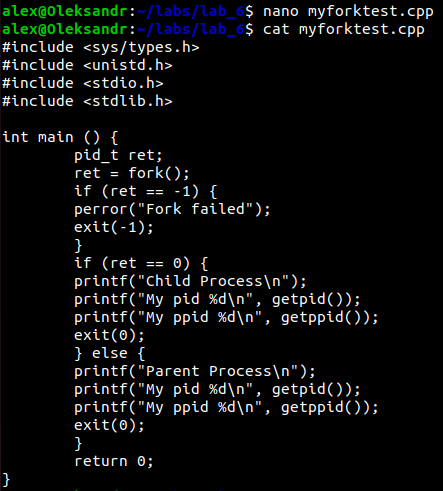
\includegraphics[width=0.6\linewidth]{Prt sc/Figure_1.png}  
        \end{minipage}
    \end{figure}
    \begin{center}
        \Large{Task \RomanNumeralCaps{2}}
    \end{center}
    \textbf{Скомпілюйте програму \\
    g++ -o myforktest myforktest.cpp}
    \begin{figure}[h!]
        \begin{minipage}[h]{1\linewidth}
            \centering
            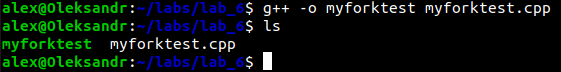
\includegraphics[width=0.6\linewidth]{Prt sc/Figure_2.png}  
        \end{minipage}
    \end{figure}

\newpage
    \begin{center}
        \Large{Task \RomanNumeralCaps{3}}
    \end{center}
    \textbf{Запустіть програму myforktest. У якій послідовності виконуються батьківський процес і процес-нащадок? Чи
    завжди цей порядок дотримується?}
    \begin{figure}[h!]
        \begin{minipage}[h]{1\linewidth}
            \centering
            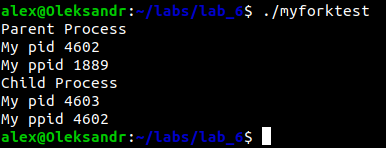
\includegraphics[width=0.6\linewidth]{Prt sc/Figure_3.png}  
        \end{minipage}
    \end{figure} \\
    <<Parent Process>> створює копію самого себе, тобто створює <<Child Process>>. Після вони продовжують виконуватися паралельно.
    Таким чином, батьківський процес завжди продовжує виконуватись першим після виклику fork(). 
    Процес-нащадок розпочинає своє виконання паралельно з батьківським процесом з того місця програмного коду, де була викликана команда.
    \begin{center}
        \Large{Task \RomanNumeralCaps{4}}
    \end{center}
    \textbf{Додайте затримку у виконання одного або обох з цих процесів (функція sleep(), аргумент — затримка у
    секундах). Чи змінились результати виконання?}
    \begin{figure}[h!]
        \begin{minipage}[h]{1\linewidth}
            \centering
            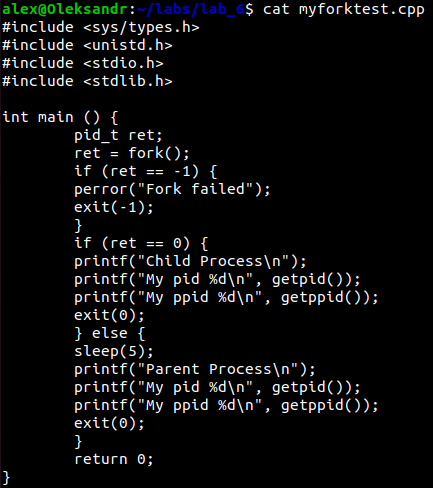
\includegraphics[width=0.6\linewidth]{Prt sc/Figure_4_1.png}  
        \end{minipage}
    \end{figure}

\newpage
    \begin{figure}[h!]
        \begin{minipage}[h]{1\linewidth}
            \centering
            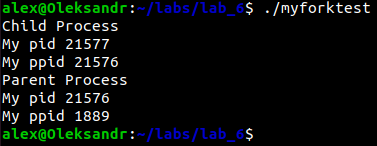
\includegraphics[width=0.6\linewidth]{Prt sc/Figure_4_2.png}  
        \end{minipage}
    \end{figure}
    Затримка у виконанні одного з процесів не вплине на порядок запуску процесів. 
    Батьківський процес все одно розпочне виконання першим, а процес-нащадок - після того, як батьківський процес створить його за допомогою функції fork().
    Проте, якщо функція sleep() викликається в процесі-нащадку, то процес-нащадок буде зупинений на визначений період часу, що може вплинути на загальний час виконання батьківського процесу, оскільки батьківський процес буде чекати, доки процес-нащадок відновить свою роботу після затримки.
    \begin{center}
        \Large{Task \RomanNumeralCaps{5}}
    \end{center}
    \textbf{Додайте цикл, який забезпечить кількаразове повторення дій після виклику fork(). Які результати показують
    процеси (значення глобальної змінної і змінної, що визначена у стеку)? Поясніть.}
    \begin{figure}[h!]
        \begin{minipage}[h]{1\linewidth}
            \centering
            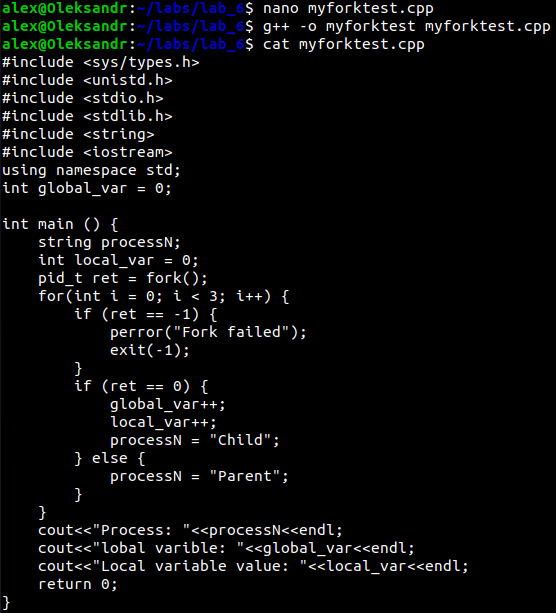
\includegraphics[width=0.6\linewidth]{Prt sc/Figure_5_1.png}  
        \end{minipage}
    \end{figure}

\newpage
    \begin{figure}[h!]
        \begin{minipage}[h]{1\linewidth}
            \centering
            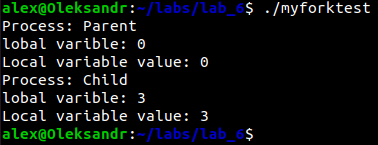
\includegraphics[width=0.6\linewidth]{Prt sc/Figure_5_2.png}  
        \end{minipage}
    \end{figure}
    Для батьківського процесу будемо мати порожні значення змінних. Після створення дочірнього процесу він пробіжить по циклу три рази й додасть до цих змінних по одиниці за один прохід.
    Тому пілся виконання коду бачимо, що значення в дочірньому процесі змінились від нуля до трьох.
    \begin{center}
        \Large{Task \RomanNumeralCaps{6}}
    \end{center}
    \textbf{Спробуйте у первинній програмі (без циклу) замість виклику fork() здійснити виклик vfork(). У чому різниця
    роботи цих двох викликів? Чи виникає помилка (якщо так, то яка)? У чому причина? Як “змусити” працювати виклик
    vfork()? Які результати тепер показують процеси (значення глобальної змінної і змінної, що визначена у стеку)? Поясніть.}
    \begin{figure}[h!]
        \begin{minipage}[h]{1\linewidth}
            \centering
            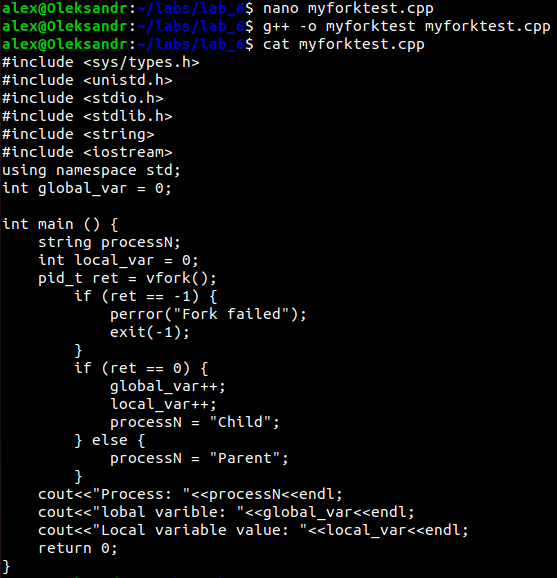
\includegraphics[width=0.6\linewidth]{Prt sc/Figure_6_1.png}  
        \end{minipage}
    \end{figure}

\newpage
    \begin{figure}[h!]
        \begin{minipage}[h]{1\linewidth}
            \centering
            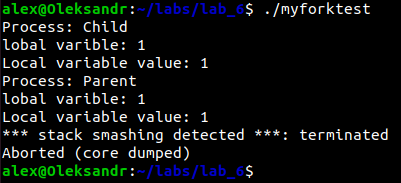
\includegraphics[width=0.6\linewidth]{Prt sc/Figure_6_2.png}  
        \end{minipage}
    \end{figure}
    fork() створює новий процес шляхом копіювання вмісту батьківського процесу (включаючи вміст змінних ). 
    vfork() створює новий процес, але він використовує спільні змінні з батьківським процесом без його копіювання.
    Також виклик vfork() блокує батьківський процес до тих пір, поки дочірній процес не викличе одну з функцій з exec.

    Так, виникає помилка "stack smashing detected: terminated. Aborted (core dumped)". 
    vfork() створює дочірній процес, який не завершує своє виконання, тому отримали помилку переповнення стеку.
    Для вирішення цієї проблеми достатньо завершити виконання дочірнього процесу за допомогою команди exit(0);
    \begin{figure}[h!]
        \begin{minipage}[h]{1\linewidth}
            \centering
            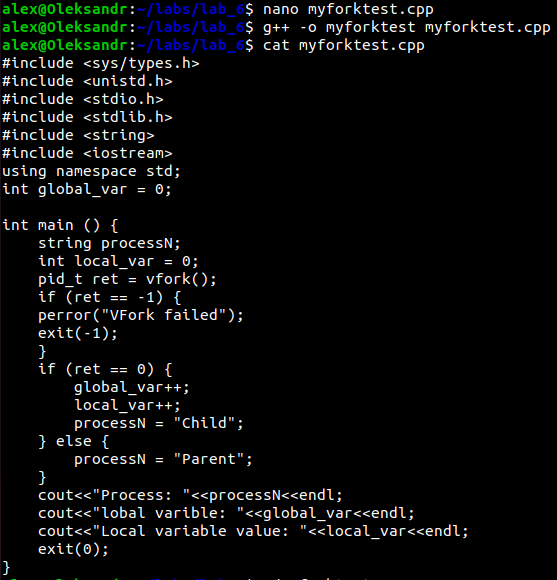
\includegraphics[width=0.5\linewidth]{Prt sc/Figure_6_3.png}  
        \end{minipage}
    \end{figure}
    \begin{figure}[h!]
        \begin{minipage}[h]{1\linewidth}
            \centering
            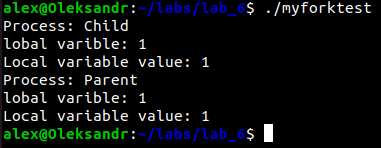
\includegraphics[width=0.5\linewidth]{Prt sc/Figure_6_4.png}  
        \end{minipage}
    \end{figure} 

    Оскільки дочірній процес було створено командою vfork(), можемо побачити, 
    що він змінив значення глобальної та локальної змінної на одиницю. Оскільки адресний простір вони мають однаковий, тому і значення для двух процесів рівні.

\newpage
    \begin{center}
        \Large{Task \RomanNumeralCaps{7}}
    \end{center}
    \textbf{Тепер додайте виклик exec() у код процесу-нащадка. Для початку використайте простішу функцію execl(). Варіант
    виклику на прикладі утиліти ls: \\
    \textbf{execl("/bin/ls", "/bin/ls", "-a", "-l", (char *) 0);} }
    \begin{figure}[h!]
        \begin{minipage}[h]{1\linewidth}
            \centering
            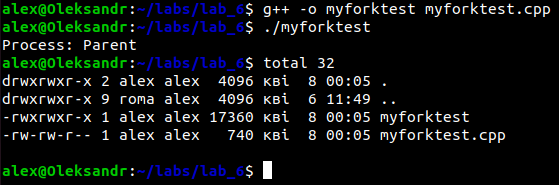
\includegraphics[width=0.6\linewidth]{Prt sc/Figure_7.png}  
        \end{minipage}
    \end{figure}
    \begin{center}
        \Large{Task \RomanNumeralCaps{8}}
    \end{center}
    \textbf{Проведіть експерименти з викликом різних програм, у тому числі ps, bash, а також з викликами execl() у
    батьківському процесі. Як запустити фоновий процес-нащадок? Як процес-нащадок дізнається власний PID? PID батьківського процесу?}
    \begin{figure}[h!]
        \begin{minipage}[h]{1\linewidth}
            \centering
            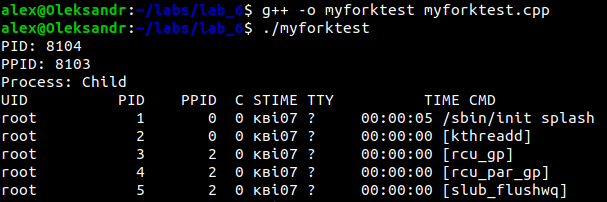
\includegraphics[width=0.6\linewidth]{Prt sc/Figure_8_1.png}  
        \end{minipage}
    \end{figure}
    \begin{figure}[h!]
        \begin{minipage}[h]{1\linewidth}
            \centering
            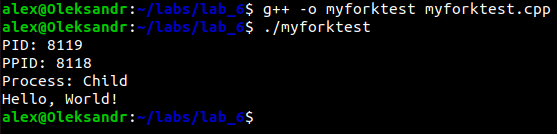
\includegraphics[width=0.6\linewidth]{Prt sc/Figure_8_2.png}  
        \end{minipage}
    \end{figure}
    \begin{figure}[h!]
        \begin{minipage}[h]{1\linewidth}
            \centering
            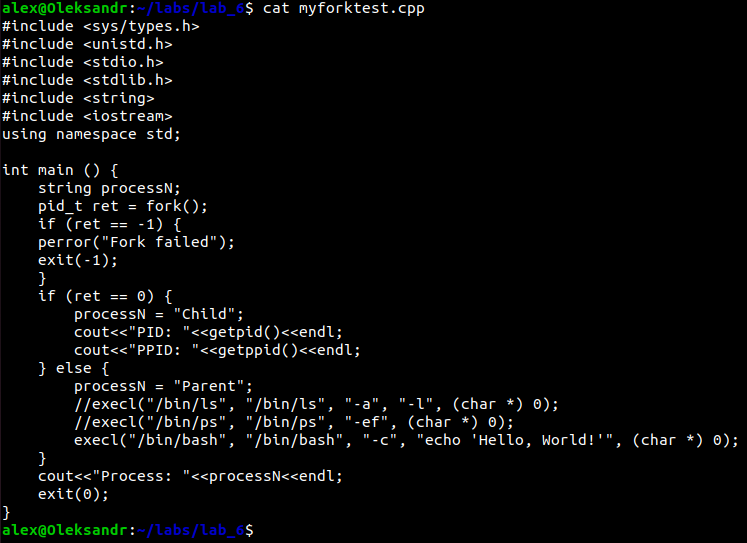
\includegraphics[width=0.5\linewidth]{Prt sc/Figure_8_3.png}  
        \end{minipage}
    \end{figure}

\newpage
    Щоб перевести процес-нащадок в фоновий режим, можемо скористатись такими командами:
    \begin{enumerate}
        \item Використання символу "\&" в кінці команди. \\
        \textbf{./my\_program \&}
        \item Використання команди "nohup". \\
        \textbf{nohup ./my\_program \&}
    \end{enumerate}

    Новий процес-нащадок, який створюється з батьківського процесу, отримує свій власний унікальний ідентифікатор процесу (PID), 
    який відмінний від PID процесу-батька. Проте PPID він буде мати такий самий, як і PID батьківського процесу.
    \begin{center}
        \Large{Висновки}
    \end{center}

    Процес забезпечує взаємодію між програмами в UNIX-подібних системах. Системні виклики fork() і exec() дозволяють створювати нові процеси та керувати їх роботою.

    Системний виклик fork() дозволяє створювати дочірні процеси, які є копіями батьківського процесу. Дочірній процес має власну пам'ять і ресурси.

    Системний виклик exec() дозволяє замінити вміст поточного процесу новим процесом. Тобто дозволяє виконувати нові програми в поточному процесі, зберігаючи при цьому його ідентифікатор процесу (PID) і ресурси.

    Комбінація викликів fork() і exec() дозволяє створювати програми, які можуть комбінувати різні функції і взаємодіяти між собою.

    Важливо також звернути увагу на обробку помилок при використанні системних викликів fork() і exec().
    Оскільки неправильна послідовність викликів може призвести до втрати даних або некоректної роботи програми.
    
    Узагальнюючи, розуміння процесів дозволяє забезпечити ефективну взаємодію між різними компонентами програми та оптимальне використання ресурсів системи. 
    Ці навички також можуть бути корисними при розробці системних додатків, демонів, серверів та інших програм, де потрібно контролювати багатопроцесову роботу.

\end{document}